\chapter{Background and Related Work}
\label{ch:background}
In the following chapter, we introduce all significant entities and tools adopted by the MMK Driving Simulator. Moreover, we discuss other research which is similar to the currently presented project. The simulator itself is implemented in Unity3D\cite{unity}, while all of the 3D models and textures are generated by ESRI CityEngine\cite{ce}. Additionally, the map information is exported from OpenStreetMap\cite{osm} and the traffic simulation is accomplished using SUMO Engine\cite{sumo}. We discuss essential characteristics of these tools which are later used to achieve the goals described in Chapter \ref{ch:introduction}. 

\section{Related Work}
Many research about semantic description of urban street network has already been conducted in the recent years. Haubrich \emph{et al.} has developed a workflow for rapid 3D traffic scenario generation\cite{haubrich2013semantic}. They use OpenStreetMap (OSM) data and generate the necessary 3D shapes and road description in OpenDRIVE\cite{dupuis2010opendrive} format using \emph{Trian3D Builder}. Both, the shapes and the description are imported into Unity3D. The aim was the creation of a road network that can be used for traffic simulation, as part of the AVeSi project ("Agentenbasierte Verkehrssimulation"). Shi has also implemented a tool in his master thesis\cite{shi2011automatic} which converts OSM data in OpenDRIVE format. However, the tool is not integrated with a 3D building environment and choses to interpolate the OSM data using standard techniques which may not coincide with separately generated 3D shapes. Lastly, in 2010, Hiblot \emph{et al.} presented ROADS\cite{hiblot2010pro}, a procedural modelling application for road networks. ROADS offers the possibility to draw roads on a 2D map and export their semantic description.  

\section{OpenStreetMap}
\label{ch:osm}
OpenStreetMap (OSM) is a open source project that creates and distributes free geographic data for the world. The project was created by the OpenStreetMap Foundation and it is completely supported by volunteers. OSM represents physical features on the ground (\emph{e.g.}, roads, buildings) using tags attached to its basic data structures: \texttt{nodes}, \texttt{ways}, and \texttt{relations}. Each tag describes a geographic attribute of the feature being shown by that specific OSM object. Among other attributes, each basic data structure of OSM has a \texttt{64 bit} integer identification number (\emph{OSM-ID}), which allows every object to be uniquely identifiable.

A \texttt{node} represents a specific point on the earth's surface defined by its coordinates in the WGS-84 coordinate system (latitude and longitude). They can be used to define standalone point features \emph{e.g.} park bench or a water well or they could define the shape of a way. A \texttt{way} is an ordered list of between 2 and 2,000 nodes that define a polyline. Ways are used to represent linear features such as rivers and roads, as well as boundaries of areas such as buildings. Finally, a \texttt{relation} is a multi-purpose data structure that documents a relationship between two or more data elements, \emph{e.g.} route relation.

There exist a possibility to export a certain area of the map in an \texttt{xml} format which can be easily parsed or visualised with different tools, \emph{e.g.} \emph{JOSM}\footnote{\url{https://josm.openstreetmap.de}} 

\section{ESRI City Engine}
\label{ch:ce}
\emph{ESRI CityEngine} (CE) is a three-dimensional modelling software application developed by \emph{Esri R\&D Center Zurich} and is specialised in the generation of 3D urban environments (Figure \ref{fig:ce-2}). There are multiple possibilities to create a city model with CE. On the one hand, one could import a third-party (2D) map data, such as OSM described in the previous section or 3D models in \texttt{.shp} or \texttt{.fbx} format. Afterwards, the application will try to generate 3D models using the 2D data and additional information (\emph{e.g.} defined tags for every OSM basic data structure) and specified by the user rules. Finally, the resulting shapes can be exported to commonly used formats such as \texttt{.obj} or \texttt{.fbx}.

\begin{figure}[htb]
	\centering
	\subfigure[] {
	  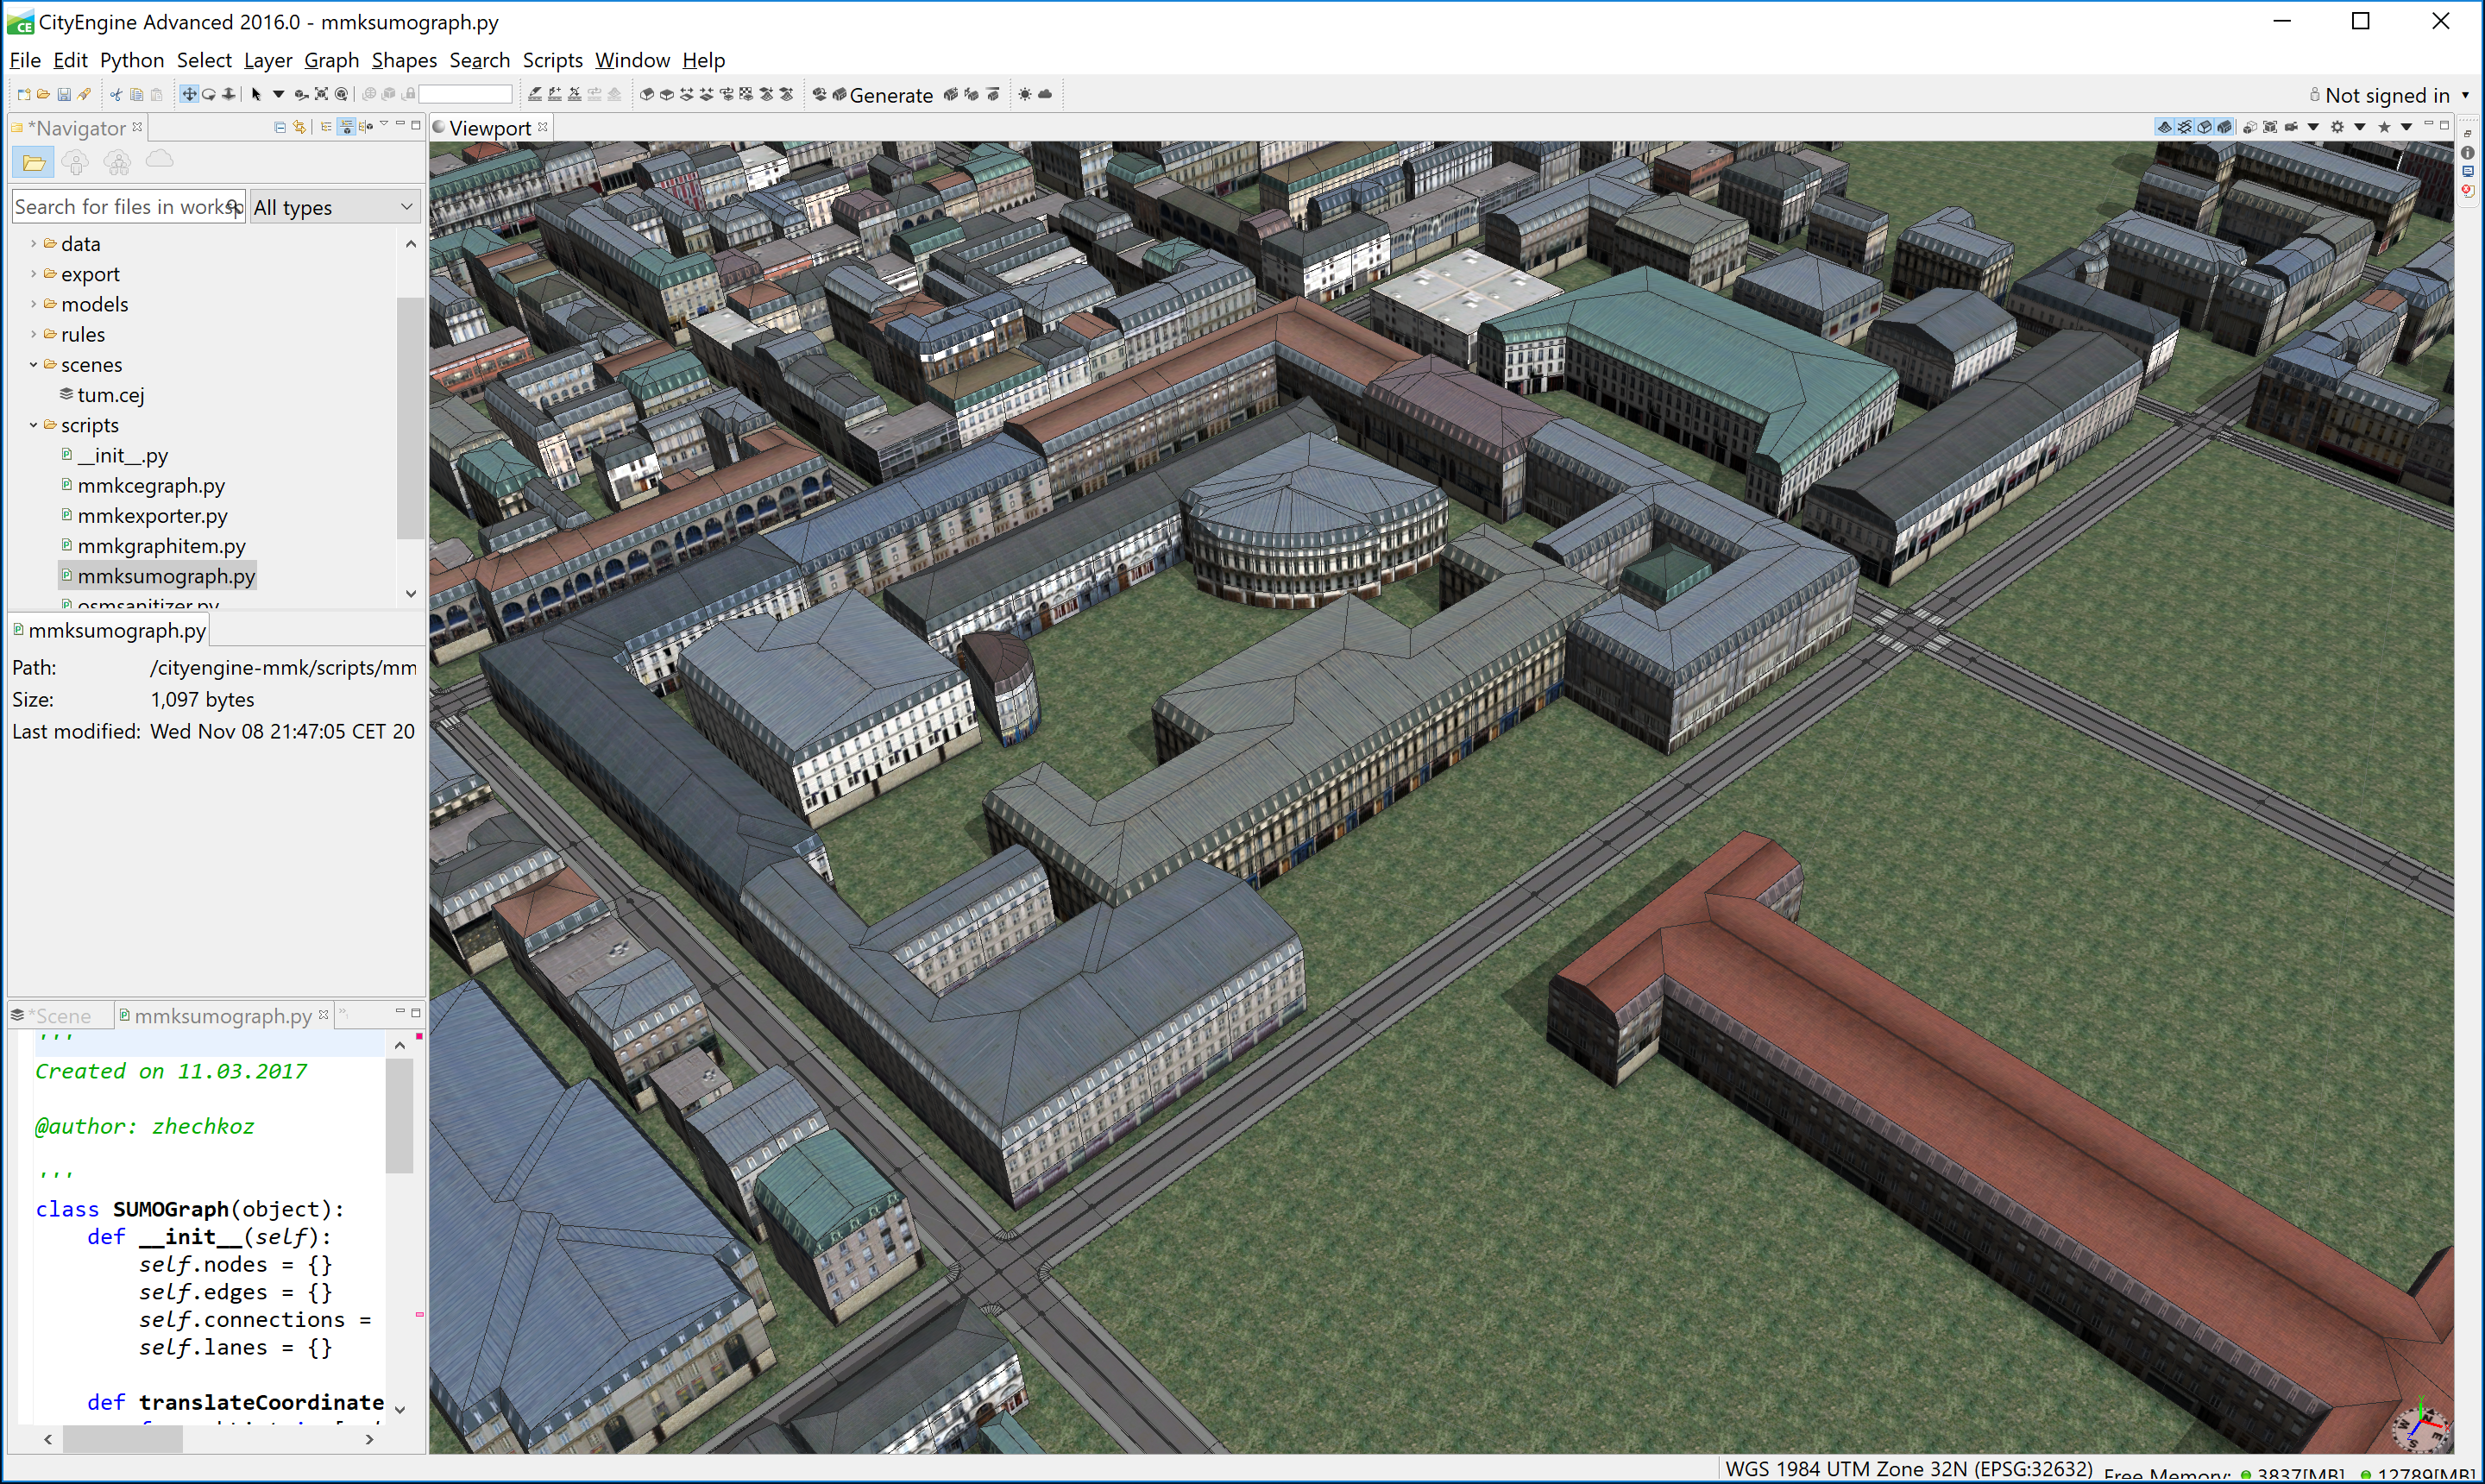
\includegraphics[width=0.66\textwidth]{figures/ce-2}
	  \label{fig:ce-2}
	}%\hspace{0.05\textwidth}% \hfill or \hspace{5mm} or \hspace{0.3\textwidth}
	\subfigure[] {
	  \includegraphics[width=0.3\textwidth]{figures/export}
	  \label{fig:export}
	}
	\caption{Finished CityEngine scene on the left (a) and the export window on the right(b), where with red is marked the \emph{Center} button.}
\end{figure}

The coordinate system used to represent the location of all objects in the scene is a \texttt{y}-up left-handed 3D cartesian coordinate system\cite{ceman}. In the case of map data imported from OSM, the position of every object in the city model is determined by their own WGS-84 (\texttt{(a, b, 0)}) coordinates projected in the Universal Transverse Mercator (UTM) \texttt{z}-up coordinate system (\texttt{(a, b, 0)}). However, the WGS-84 coordinates are just 2D values, therefore, CE utilises many attributes, defined in the OSM export, in order to interpolate a third dimensional position of each object (\texttt{(a, b, c)}). But this is still a \texttt{z}-up coordinate system. In order to convert all coordinates to a \texttt{y}-up coordinate system, CE applies a rotation by \texttt{-90$^{\circ}$} and as a result we have \texttt{(a, c, -b)}. If one would like to find locations of OSM objects in CE, they have to use a third-party library for WGS-84/UTM conversion (\emph{e.g.} \texttt{utm}\cite{utm}), as well as follow the aforementioned process. Nevertheless, the \texttt{y} cannot be generated correctly because of internal CE routines which are not widely accessible. When exporting 3D models from CE to one of the compatible formats, one could center the whole scene automatically (as can be seen in Figure \ref{fig:export}), so the origin of all models is located at the origin \texttt{(0, 0, 0)}.

The generated street network model is composed of \texttt{segments} and \texttt{nodes}. Each node is defined by one 3D point in the scene, while each segment composes of exactly two nodes which define its form. Both, nodes and segments, have unique ID (\texttt{OID}) and can hold shapes as children objects, which are referenced with the same ID as their parent segment or node and an index (\texttt{OID:INDEX}). Maximilian Murauer[*] has already implemented a Python script in his research project at the Institute of Human-Machine Interaction, TUM which exports the properties of all nodes, segments and their corresponding shapes in JSON format. However, this was never imported in the Driving Simulator.

CE includes a \texttt{Jython} interface which can be utilised to access and change scene's objects properties. CE 2016 uses \texttt{Jython 2.7b21}, which already has the most common Python modules, however there are some necessary software which has to be manually included to the \texttt{Jython} environment. In order to use the export scripts which will be described in the next chapter, one have to download and copy \texttt{simplejson} folder to \texttt{C:$\backslash$Users$\backslash$<USERNAME>$\backslash$.CityEngine$\backslash$2016.0R.win32.win32.x86\_64$\backslash$jythonCache$\backslash$\\ThirdParty}.

\section{Simulation of Urban MObility (SUMO)}
\label{ch:sumo}
SUMO is a open-source (licensed under the GPL) traffic simulation software which was developed by the National Aeronautics and Space Research Center of the Federal Republic of Germany in Berlin. It is highly portable, microscopic (\emph{i.e.} each vehicle is controlled separately) and continuous (\emph{i.e.} runs in predefined steps) road traffic simulation package designed to handle large road networks. SUMO's traffic simulation runs in separate steps where each vehicle, by following its \emph{lane}, is moved to the next destination. However, some of these actions, such as lane switching are accomplished not in a smooth fashion. Before the simulation begins one has to define the geometry and the properties of the street network, as well as each vehicles's characteristics. This is realised by generating a couple of \texttt{xml}-based configuration files. In the following section, we will describe some of the most relevant to this project fields from \texttt{net.xml} file.

Firstly, \texttt{net.xml} describes the whole street network using five main objects: \texttt{location}, \texttt{junction}, \texttt{edge}, \texttt{lane}, \texttt{connection}. This configuration file can be generated using \texttt{netconvert} tool which is available in the SUMO package from many input formats, \emph{e.g.} \emph(OSM Export Format), \emph{OpenDRIVE}. Additionally, the final \texttt{net.xml} can be illustrated using SUMO's GUI tool (Figure \ref{fig:sumo}). There are many options which can be passed to \texttt{netconvert} either by command line or as a configuration file. Using these options, one could customise the street network generation process. To generate all necessary \texttt{net.xml} files in this project we used two optional parameters which were passed to \texttt{netconvert}: \texttt{output.street-names true} and \texttt{output.original-names true}, which preserve the original OSM information. SUMO adopts again a new custom coordinate system which uses translation and projection to convert the original objects' coordinates. This is done in such a way that the left, top corner of the scene has the coordinates \texttt{(0, 0)}. The applied transformation and projection parameters can be found in the \texttt{location} tag. CE and SUMO usually use the same parameters for the  projection but they differ in their choice of translation values for each object in the scene.

The most substantial object in the \texttt{net.xml} file for this project is \texttt{edge}. It holds an information about the track between two nodes, which is equivalent to a \texttt{segment} in CE. There are generally two types of \texttt{edges}: \emph{internal} and \emph{ordinary}. The latter specify the connection between two junctions. The important attributes of this kind of \texttt{edge} are \texttt{id}, which is a unique identification of a street. If the source of the map data is OSM, then this \texttt{id} has the form \texttt{OSM-ID\#INDEX}, where \texttt{INDEX} is necessary since it is possible that one \texttt{way} in OSM to correspond to more than one \texttt{edge} in SUMO. Next, \texttt{edge} has \texttt{from} and\texttt{to} attributes which specify its start and end node. Lastly, the \emph{internal} type of \texttt{edge} define a node. In this case the \texttt{id} has the form \texttt{:OSM-ID\#INDEX} and \emph{function} is marked as \emph{internal}. Both \texttt{edge}-types posses \emph{lanes} as child nodes.

As already mentioned \texttt{edge} contains a list of lanes, which specify the actual vehicle's driving lanes. One lane always corresponds to exactly one \texttt{edge}. Lane's attributes which are beneficial for this project are \texttt{id}, \texttt{index}, which represents the position of the lane on the street, \texttt{length} and \texttt{shape}. If the map data are imported from OSM then the \emph{id} of a lanes has the following format \texttt{OSM-ID-of-parent-edge\_INDEX}. All \texttt{shape} values are defines as space-separated list of 2D points (\texttt{x} and \texttt{y} values separated again by a comma).

\begin{figure}[htb]
	\centering
	\subfigure[] {
	  \includegraphics[width=0.47\textwidth]{figures/sumo}
	  \label{fig:sumo}
	}%\hspace{0.05\textwidth}% \hfill or \hspace{5mm} or \hspace{0.3\textwidth}
	\subfigure[] {
	  \includegraphics[width=0.47\textwidth]{figures/unity}
	  \label{fig:unity}
	}
	\caption{SUMO (a) and Unity (b) interface.}
\end{figure}

Finally, \texttt{connections} in \texttt{net.xml} facilitate the description of links between different \texttt{edges}. There are multiple metadata options which ease the driving of vehicle through the connections. Moreover, the connections are built according to the driving law. By employing the connectivity information between the lanes one could construct a path from one point on the street network to another. The most prominent connection's attributes are \texttt{from/to}, \texttt{fromLane/toLane} and \texttt{via} (possible intermediate lanes which has to be driven through in order to reach the destination lane). 

\section{Unity}
\label{ch:unity}
As previously mentioned the MMK Driving Simulator has currently been developed  in Unity3D \texttt{v5.6.3} which uses \texttt{dotNet v4}. In the following, we highlight the most prominent conjunctions of Unity and the rest of the software introduced in this chapter. Moreover, we discuss the necessary extension which has to be added to Unity in order to utilise them later in this project.

The generated urban network together with the 3D models can be exported from CE and imported in Unity using the following steps: (1) Create folder \texttt{Assets$\backslash$Models$\backslash$<name of scene>}, (2) Create folder \texttt{Assets$\backslash$Models$\backslash$<name of scene>/Textures} and copy all pictures from models folder in CityEngine to this folder, (3) Copy the exported file (\emph{e.g.} \texttt{.fbx}) file to \texttt{Assets$\backslash$Models$\backslash$<name of scene>} (the materials folder will be created automatically). These steps has to be executed in the presented order so the textures are added automatically to all models. Finally, if the format of the exported model from CE is \texttt{fbx}, all objects in the Unity scene has to be scaled in all directions with \texttt{100}. An example result can be seen in Figure \ref{fig:unity}.

In this project we utilise Dijkstra's Algorithm to find the shortest path between two lanes in the street network. As explained in Chapter \ref{ch:gps}, we need a priority queue which will always track the nearest lane according to the currently visited lane. Unfortunately, the used version of Unity does not implement a priority queue in their standard library. In fact, one could use \texttt{Dictionary} and the \texttt{Sort} method to implement a priority queue. However, there exist a open-source \emph{High Speed Priority Queue for C\#}\cite{pq} implemented by BlueRaja and licensed under \emph{MIT}. The project is referenced in multiple Unity3D forums and has also a big star rating on GitHub. By default, the \texttt{SimplePriorityQueue.cs} class uses float numbers to manage priority of elements but in the Driving Simulator we use double precision numbers to measure the distances. Therefore, before using it, one have to change all occurrences of \texttt{float} with \texttt{double}.

Another third-party software which was necessary for the project is \emph{SimpleJSON} C\# script which can be found on UnityWiki. The format we have chosen for the semantic description of the street network is JSON but Unity3D API does not natively support it. Therefore, we had to find an implementation of a JSON parser and \emph{SimpleJSON} was pointed out again as a considerable option.
